\documentclass[a4paper,12pt]{report}
\usepackage{color}
\usepackage{hyperref}
\hypersetup{
    colorlinks,
    citecolor=black,
    filecolor=black,
    linkcolor=black,
    urlcolor=blue
}
\setcounter{tocdepth}{4}
\setcounter{secnumdepth}{0}
\usepackage{graphicx}
\usepackage{epstopdf}
\epstopdfsetup{outdir=./}	
\usepackage{amsmath}
\usepackage[table,xcdraw]{xcolor}
\usepackage{amssymb}
\usepackage{listings}
\definecolor{anti-flashwhite}{rgb}{0.95, 0.95, 0.96}
\lstset{
	language=C++,
    basicstyle=\ttfamily,
    keywordstyle=\color{blue}\ttfamily,
    stringstyle=\color{red}\ttfamily,
	commentstyle=\color{green}\ttfamily,
    morecomment=[l][\color{magenta}]{\#},
    backgroundcolor=\color{anti-flashwhite}
}
\begin{document}
\title{
\textbf{Computer Networks I: CS3530}\\~\\
\begin{large}
\textbf{Programming Assignment I \& II \\Socket Programming}\\~\\
\end{large}
\begin{large}
\textbf{Assignment Report}
\end{large}
}
\author{\textbf{Sagar Jain - CS17BTECH11034}\\}
\maketitle
\begin{large}
\tableofcontents
\end{large}
\newpage
\section{Assignment I}
\subsection{Question I}
\subsection{Feature I: Interactive Server \& Persistent Client}
The following has been achieved:
\begin{enumerate}
\item The client does not close after sending a single message, the client can keep sending messages and finally quit using \textit{bye}.
\item Clients can use HELP to know all available commands.
\item Clients are allowed to request for the time by typing in TIME.
\item Clients can query the total number of requests using NQUERY.
\item The methodology to create many more such commands is incorporated with just a simple string check and can be seemlessly extended according to the developer.
\end{enumerate}
\subsubsection{Points to note about the code}
\begin{enumerate}
\item The client was made continuous by putting the receive and send in a while loop and clearing the receive and send buffers every iteration.
\item The commands are run on server using string comparisions, and if the receive length is zero it is assumed that the client has disconnected.
\end{enumerate}
\subsubsection{Illustration}
\begin{center}
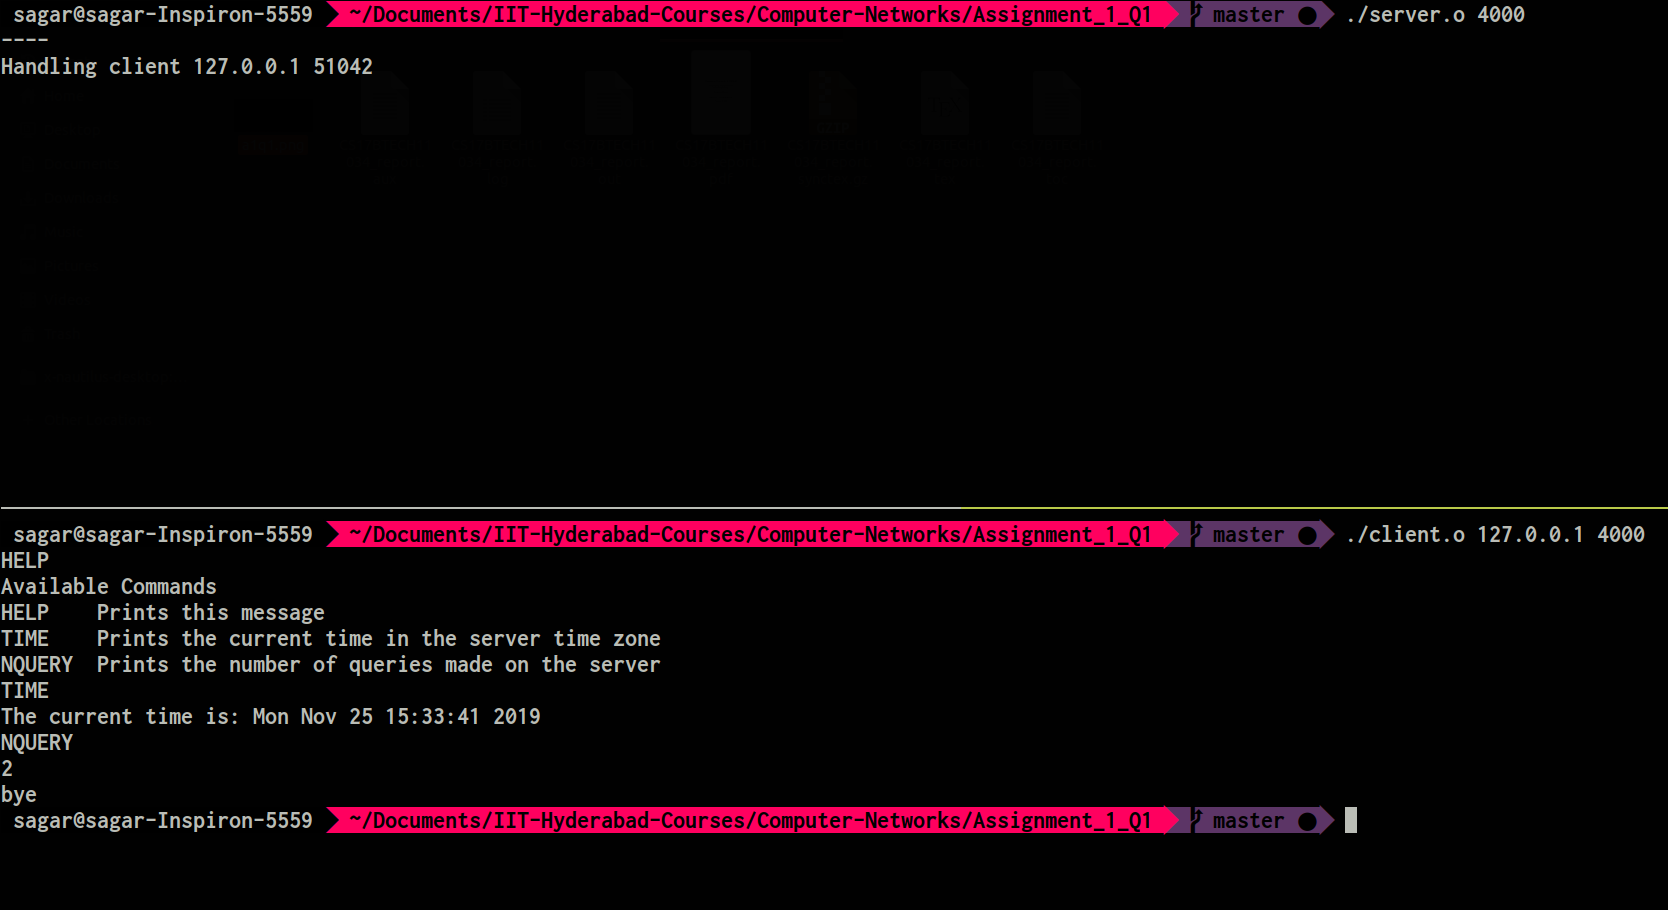
\includegraphics[scale=0.25]{a1q1f1.png}
\end{center}
\subsection{Feature II: File Transfer to Server}
The following has been achieved in this feature.
\begin{enumerate}
\item The client can select a file to send, instead of a string to send.
\item The file is received and stored on the server side.
\item New file received will not replace old files.
\end{enumerate}
\subsubsection{Points to note about the code}
\begin{enumerate}
\item The file is sent by copying the file into a string buffer.
\item The file is received into a buffer piece by piece, and put into a file on the server piece by piece.
\item This can happen because sockets work similar to file pointers and move everytime you read from them. Finally when a the entrire buffer is read the close from client side is read as a 0 length message and the server starts waiting for a new connection.
\end{enumerate}
\subsubsection{Illustration}
\begin{center}
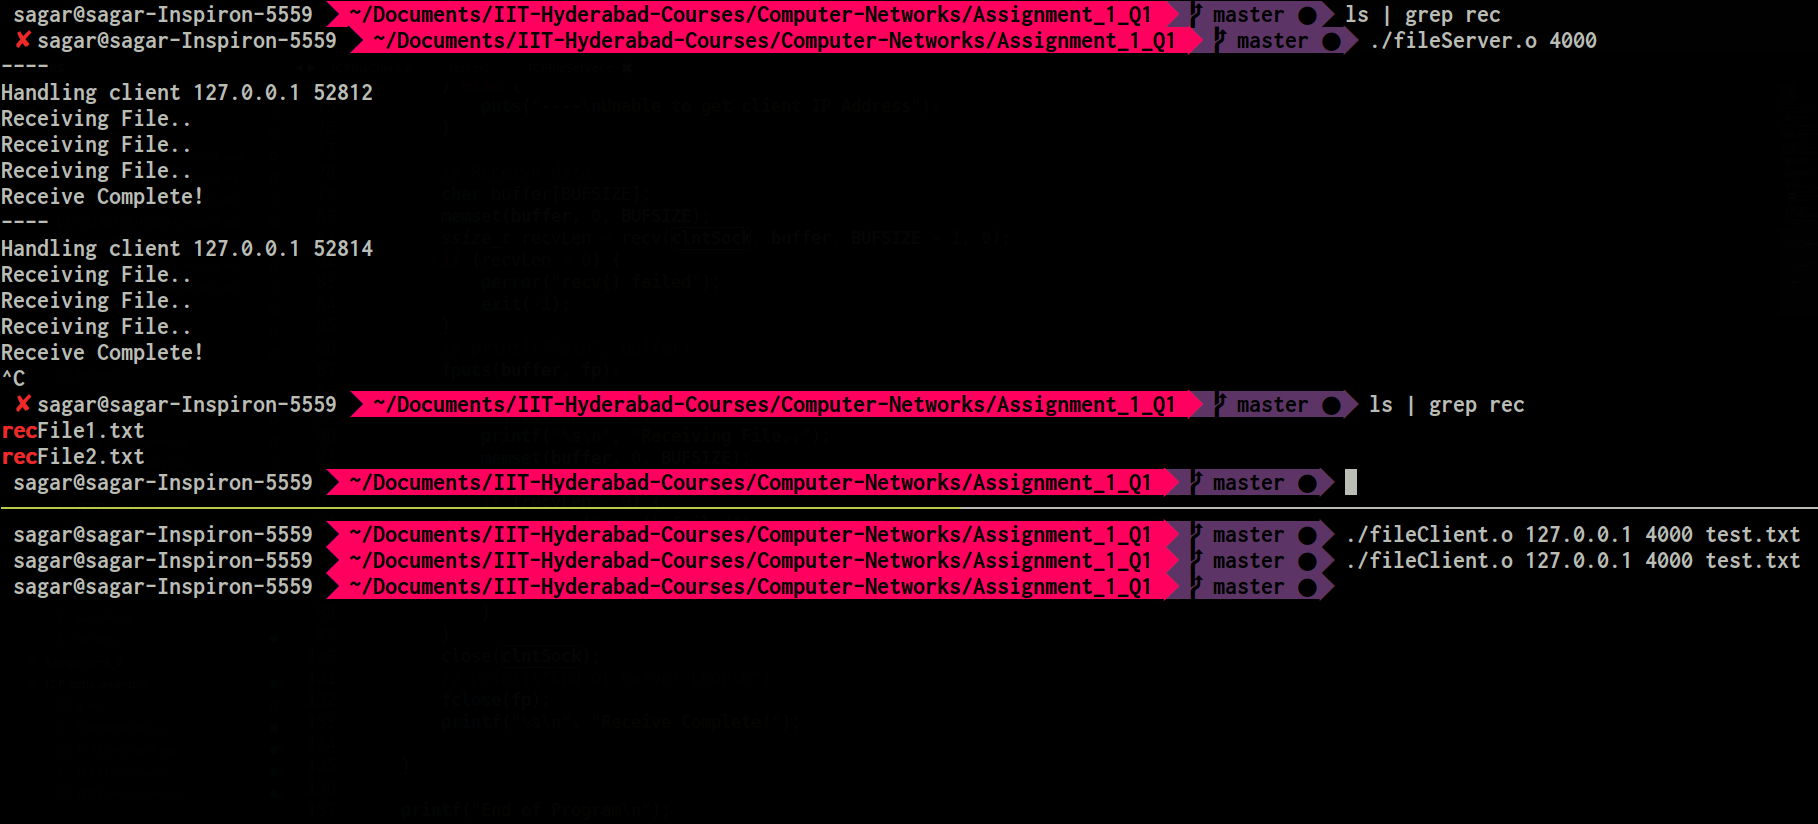
\includegraphics[scale=0.25]{a1q1f2.png}
\end{center}
\subsection{Question II}
Chosen mode is hard mode.
\subsubsection{Main Problems \& Solutions}
\begin{enumerate}
\item \textbf{How to listen and send concurrently}, it is known that while waiting for a recv you cannot use a send in C, so how do you read a message which has come from another client while the program is expecting input from you or other way how do you give input when the program is actually waiting on a recv from the server?\\
\textbf{Solution Implemented}, the answer to both the above questions that I have implemented is to use fork to have one process listen to the server always and other process to take input and send to the server always. I have used \textbf{fork} for this task, I could have used \textbf{threads} too.
\item To have the \textbf{server work with multiple clients}. This was done in the following steps:
\begin{enumerate}
\item Provide a maximum number of concurrent clients.
\item Create a \textbf{fd\_set} for all the clients.
\item Use \textbf{select} to check if any of the sockets have any activity.
\item If there is activity at the master socket implies it is a new connection.
\item If it is any of the other sockets implies they are either sending a message or have disconnected.
\end{enumerate}
\item How to allow clients to communicate with each other. \textbf{A string parsing solution}, Clients can send messages in the format where a vertical line seperates client ID and the message.
\end{enumerate}
\subsubsection{Illustration}
\begin{center}
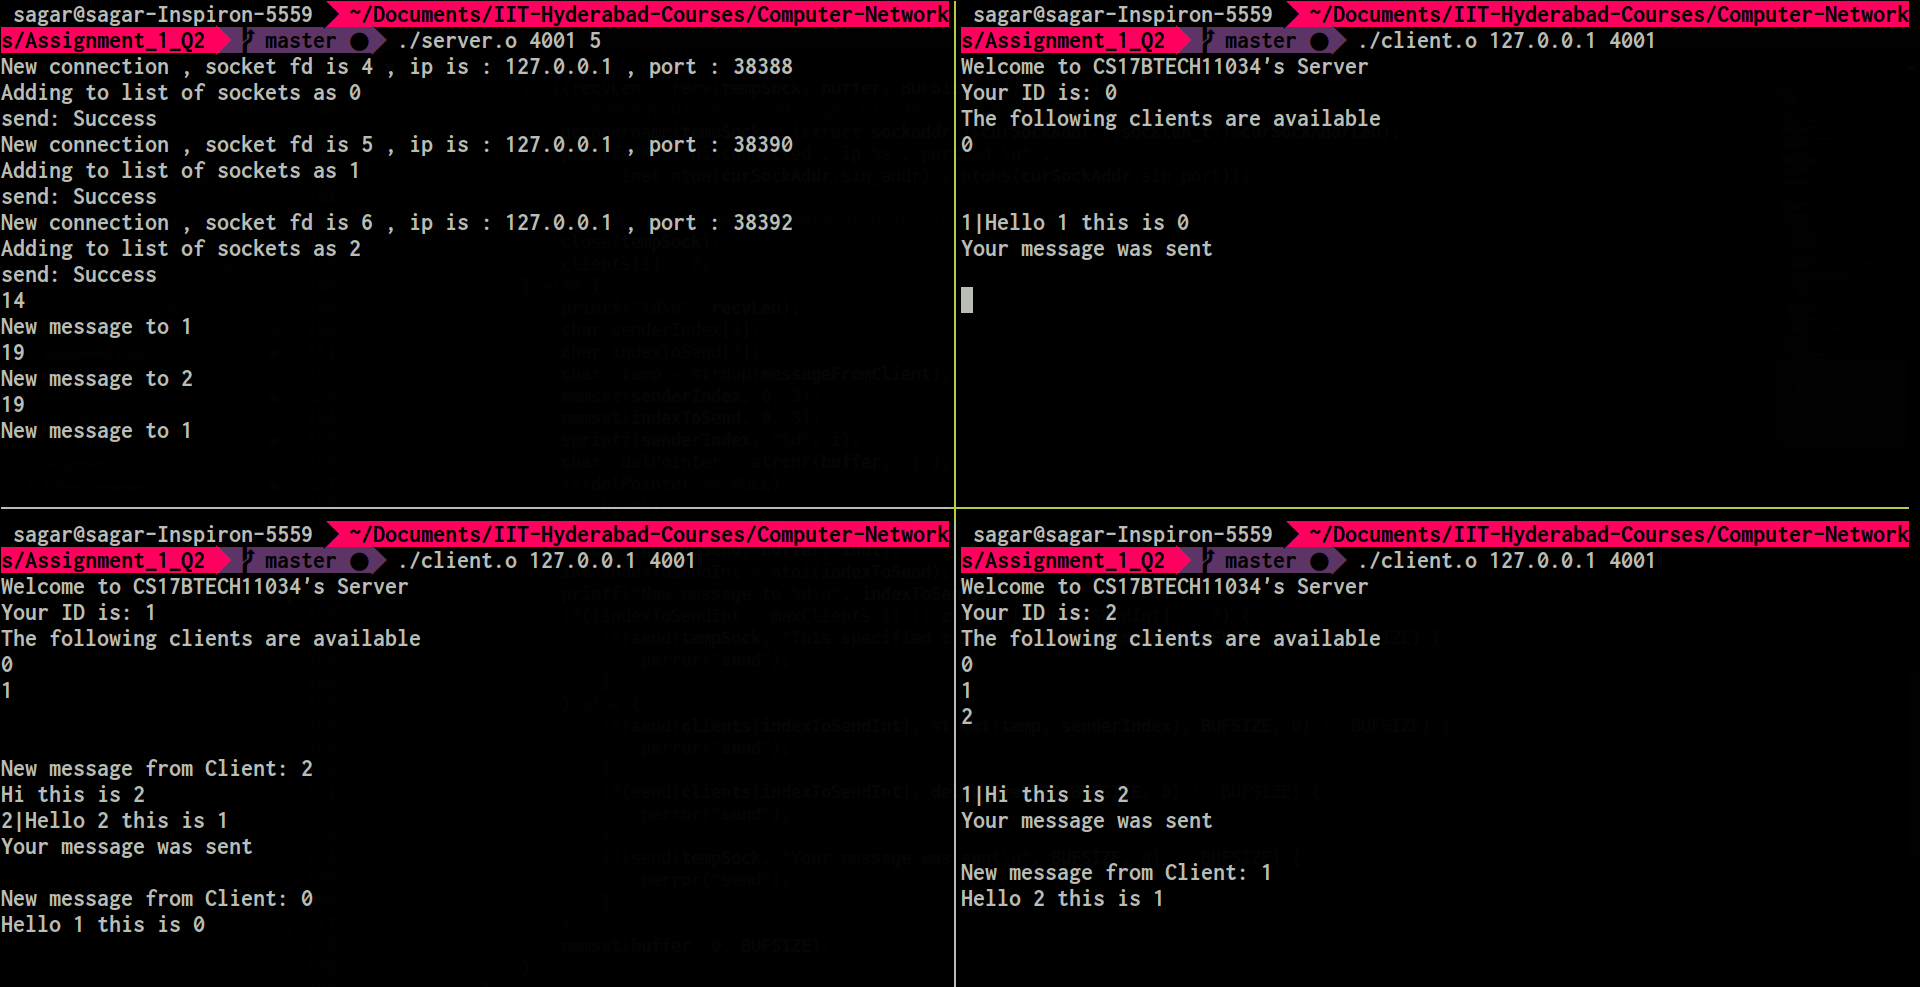
\includegraphics[scale=0.25]{a1q2.png}
\end{center}
\section{Assignment II}
\subsection{Main Problems \& Solutions}
\begin{enumerate}
\item \textbf{Get DNS working}, this is straightforward, the code from the pdf works fine to get us the \textbf{addrinfo}from which we can get the \textbf{sock\_addr}.
\item Get server to work with both IPv4 and IPv6, this can be done by mapping all IPv4 addresses to IPv6.
\item Other than this we can just use the code for the basic TCP echo server and client.
\end{enumerate}
\subsubsection{Illustration}
\begin{center}
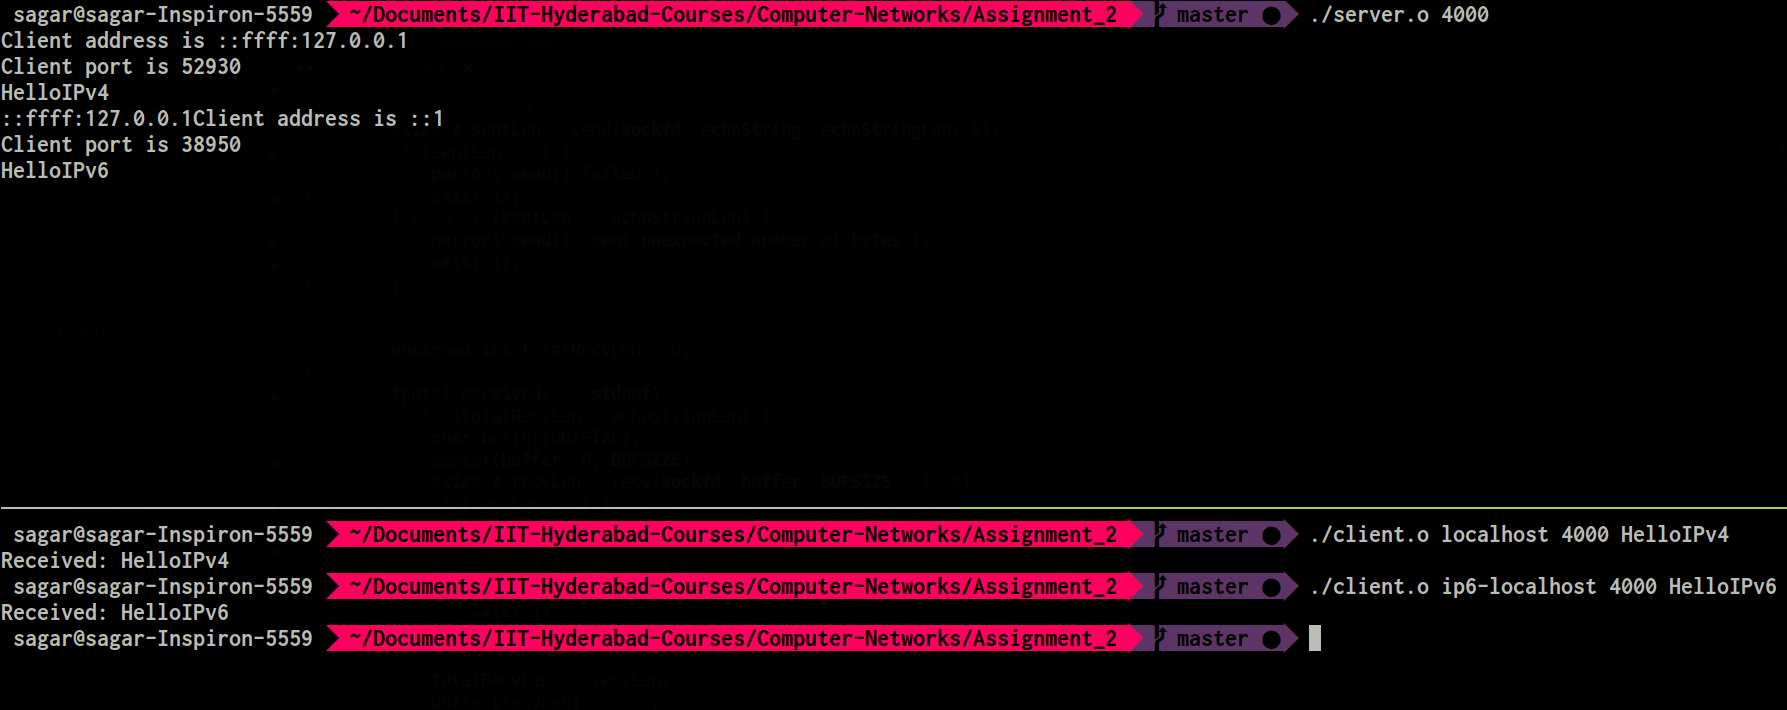
\includegraphics[scale=0.25]{a2.png}
\end{center}
\section{References}
For All
\begin{enumerate}
\item \href{https://linux.die.net/man/}{https://linux.die.net/man/}
\end{enumerate}
For Assignment 1, Question 2
\begin{enumerate}
\item \href{https://www.tutorialspoint.com/cprogramming/c\_file\_io.htm
}{https://www.tutorialspoint.com/cprogramming/c\_file\_io.htm}
\item \href{https://stackoverflow.com/questions/238603/how-can-i-get-a-files-size-in-c}{https://stackoverflow.com/questions/238603/how-can-i-get-a-files-size-in-c}
\item \href{https://www.geeksforgeeks.org/c-program-demonstrate-fork-and-pipe/}{https://www.geeksforgeeks.org/c-program-demonstrate-fork-and-pipe/}
\end{enumerate}
For Assignment 2
\begin{enumerate}
\item \href{https://www.ibm.com/support/knowledgecenter/ssw\_ibm\_i\_72/rzab6/xacceptboth.htm
CS5060\_NP.pdf}{https://www.ibm.com/support/knowledgecenter/ssw\_ibm\_i\_72/rzab6/xacceptboth.htm
CS5060\_NP.pdf}
\end{enumerate}
\end{document}